\documentclass{aiaa-tc}
\usepackage{amsmath}
\usepackage{amssymb}
\usepackage{graphicx}
\usepackage{algorithm2e}
\usepackage{float}

\title{Optimal Path Planning in the Presence of Static Obstacles and Uncertain Dynamic Obstacles}

\author{Andrew C. Campbell\thanks{Graduate Research Assistant, Aerospace Engineering \& Mechanics, accampbell4@crimson.ua.edu.}\\The University of Alabama, Tuscaloosa, AL, 35487}

\begin{document}
\RestyleAlgo{ruled}
\maketitle

\begin{abstract}
In this paper a method for augmenting the Rapidly-exploring Random Tree star (RRT*) algorithm introduced by Karaman \& Frazzoli \cite{doi:10.1177/0278364911406761} such that 
it can plan in an uncertain dynamic environment is presented. The innovation is primarily in the development of a grid management system capable of handling
multiple obstacle types including uncertian obstacles, such that the probability of a cell being occupiead at a certain time can be calculated and passed to any planning system.
Notably this grid management system is capable of interfacing with any planner that calculates its own state in relation to time as it plans. This allows for a planning algorithm to
avoid future collisions, and avoid regions that a moving obstacle could occupy in the future, all while avoind static obstacles as any conventional planner.
\end{abstract}

\section{Introduction}
The path and motion planning problem is a fundamental problem in robotics and autonomous systems.
There has yet to be an extensive amount of work done on the problem of path planning in the presence 
of dynamic obstacles,
let alone uncertain dynamic obstacles as well. 
The development then of a system that can manage all these cases
at once is necessary to provide more flexibility
for the implementation of planners on autonimous systems to run a more robust and reliable system. 
Presented here is a Grid management system that is capabel of managing certain and uncertain static obstacles
and certain and uncertain dynamic obstacles. The grid management system is capable of propagating dynamic
obstacles into the future a given amout of time with a given time step resolution and can determine the 
occupancy probability of a cell at a given time. This system cansalso sample many potential futures for a 
dynamic obstalce based on the random paramaters and boundary condistions of said obstacle. By managing 
all of this within the grid management system, it can interface with any planner that calculates its time 
of travel to a node such that it can access the grid as it plans to ensure safe planning in a dynamic uncertain environment.
To demonstrate the effectiveness of this system, the an RRT* algorithm that follow a set velocity to determine time
is paired with a path validation system that checks a bounding box for the size a vehicle for intersections with grid elements at
the desired time.

\section{Problem Definition}
Let \(\mathcal{X} \in \mathbb{R}^{n \times 1}\) where  \( n \in \mathbb{N} \) denote the \(n\)-dimensional space and one time dimension configuration space that a vehicle is operating within. 
\(\mathcal{X}_{obs} \in \mathcal{X}\) denotes the set of occupied space and time. 
\(\mathcal{X}_{free} = \mathcal{X} \setminus \mathcal{X}_{obs}\) denotes the set of free space and time. 
Let the initial state and goal be denoted by \(x_{init}, x_{goal} \in \mathcal{X}_{free}\) respectively. 

Define the vehicle \(V\) as the space confined by a polygon \(V_{poly}\) with vertices \(\{v_1, v_2, \ldots, v_n\}\) in \(\mathbb{R}^n\). 
The position and orientation of the vehicle at any time \(t\) can be represented by a transformation \(T(x, V)\), 
where \(x\) is a state in \(\mathcal{X}\) and \(T(x, V)\) is a translation and rotation applied to \(V\). 
The transformed vehicle \(V_{transformed} = T(x, V)\) represents the space aligigned with the vehicle's position and orientation in the 
configuration space \(\mathcal{X}\). Note that for path planning to be possible \(T({x_{init}, x_{goal}},V) \in \mathcal{X}_{free}\) must be true.

A dynamic obstacle \(O\) can be defined similarly to a vehicle as the space with a polygon \(O_{poly}\) with vertices \(\{o_1, o_2, \ldots, o_n\}\) 
in \(\mathbb{R}^n\) with dynamics that define some state function \(x_{obs}(t)\). 
Then, \(\mathcal{X}_{obs} \supset T(x_{obs}(t), O)\). 

An Uncertain dynamic obstacle can mean that the polygon defining the obstacle \(O_{poly}\) is not known exactly and/or the
the state function \(x_{obs}(t)\) is a function of random variables. In this case we define a new \(\mathcal{X}_{uncertain} \in \mathcal{X}\) 
for spaces that have a nonzero but less than or equal 
to one probability of occupancy, therefore \(\mathcal{X}_{obs} \subset x_{uncertain}\).

Both static certain and uncertain obstacles can be defined in the same way as dynamic obstacles, but with a state function that is invariate with time.

The goal of a path planner is to find a path \(\mathcal{P} = \{x_1, x_2, \ldots, x_n\}\) as a list of states defined such 
that \(x_1 = x_{init}\), \(x_n = x_{goal}\), and \(T(\mathcal{P}, V) \subset \mathcal{X}_{free}\).

\section{RRT* Algorithm and Grid Management System}
For an RRT* planning algorithm let \(\mathcal{T}(\mathcal{V},E)\) define the tree where \(\mathcal{V}\) are 
the vertices and \(E\) are the edges. let \(N \in \mathbb{N}\) denote the number of samples
that that the algorithm will take to plan. a cost discrete function to some horizon \(\ell\) is conventionally defined generally as:
\[
J = c_\ell(x_\ell) + \sum_{t=0}^{\ell-1} c_t(x_t, u_t),
\]
where \(c_\ell(x_\ell)\) and \(c_t(x_t, u_t)\) are local cost functions for the discrete space and \(x\) is a state and \(u\) is an input. The first term then is the cost at the
horizon and the second term is the cost to said horizon. When applied we can define our cost function \(c(x_t, u_t)\) in any way we like
to tune or guide a planner. to follow this structer a planner will have to implement the cost function such that it is summed with all parent nodes
to the current node (the horizon) in this case.

\begin{algorithm}[H]
    \caption{RRT*}\label{alg:rrtstar}
    \KwIn{$x_{init}$, $x_{goal}$, $N$}
    \KwOut{$\mathcal{P}$ from $x_{init}$ to $x_{goal}$}
    $\mathcal{T} \gets \{x_{init}\}$\;
    \For{$i \gets 1$ \textbf{to} $N$}{
        $x_{rand} \gets \text{SampleRandomState}()$\;
        $x_{nearest} \gets \text{NearestNeighbor}(\mathcal{T}, x_{rand})$\;
        $x_{new} \gets \text{Steer}(x_{nearest}, x_{rand})$\;
        \If{$\text{Validator.CollisionFree}(x_{nearest}, x_{new})$}{
            $cost_{new} \gets $ \;
            $\mathcal{T}.\text{add\_vertex}(x_{new})$\;
            $\mathcal{T}.\text{add\_edge}(x_{nearest}, x_{new})$\;
            $X_{near} \gets \text{Near}(\mathcal{T}, x_{new}, r)$\;
            $x_{min} \gets x_{nearest}$\;
            $c_{min} \gets \text{Cost}(x_{nearest}) + \text{Cost}(x_{nearest}, x_{new})$\;
            \ForEach{$x_{near} \in X_{near}$}{
                \If{$\text{Validator.CollisionFree}(x_{near}, x_{new})$ \textbf{and} $\text{Cost}(x_{near}) + \text{Cost}(x_{near}, x_{new}) < c_{min}$}{
                    $x_{min} \gets x_{near}$\;
                    $c_{min} \gets \text{Cost}(x_{near}) + \text{Cost}(x_{near}, x_{new})$\;
                }
            }
            $\mathcal{T}.\text{add\_edge}(x_{min}, x_{new})$\;
            \ForEach{$x_{near} \in X_{near}$}{
                \If{$\text{Validator.CollisionFree}(x_{new}, x_{near})$ \textbf{and} $\text{Cost}(x_{new}) + \text{Cost}(x_{new}, x_{near}) < \text{Cost}(x_{near})$}{
                    $x_{parent} \gets \text{Parent}(x_{near})$\;
                    $\mathcal{T}.\text{remove\_edge}(x_{parent}, x_{near})$\;
                    $\mathcal{T}.\text{add\_edge}(x_{new}, x_{near})$\;
                }
            }
        }
    }
    \Return $\text{ExtractPath}(\mathcal{T}, x_{goal})$\;
\end{algorithm}

\begin{algorithm}[H]
    \caption{Validator.CollisionFree()}\label{alg:validator}
    \KwIn{$x_{head}$, $x_{tail}$, $\mathcal{G}$, $\mathcal{V}$}
    \KwOut{bool $clear$}
    $\mathcal{T} \gets \{x_{init}\}$\;
    \For{$i \gets 1$ \textbf{to} $N$}{
        $x_{rand} \gets \text{SampleRandomState}()$\;
        $x_{nearest} \gets \text{NearestNeighbor}(\mathcal{T}, x_{rand})$\;
        $x_{new} \gets \text{Steer}(x_{nearest}, x_{rand})$\;
        \If{$\text{Validator.CollisionFree}(x_{nearest}, x_{new})$}{
            $\mathcal{T}.\text{add\_vertex}(x_{new})$\;
            $\mathcal{T}.\text{add\_edge}(x_{nearest}, x_{new})$\;
            $X_{near} \gets \text{Near}(\mathcal{T}, x_{new}, r)$\;
            $x_{min} \gets x_{nearest}$\;
            $c_{min} \gets \text{Cost}(x_{nearest}) + \text{Cost}(x_{nearest}, x_{new})$\;
            \ForEach{$x_{near} \in X_{near}$}{
                \If{$\text{CollisionFree}(x_{near}, x_{new})$ \textbf{and} $\text{Cost}(x_{near}) + \text{Cost}(x_{near}, x_{new}) < c_{min}$}{
                    $x_{min} \gets x_{near}$\;
                    $c_{min} \gets \text{Cost}(x_{near}) + \text{Cost}(x_{near}, x_{new})$\;
                }
            }
            $\mathcal{T}.\text{add\_edge}(x_{min}, x_{new})$\;
            \ForEach{$x_{near} \in X_{near}$}{
                \If{$\text{CollisionFree}(x_{new}, x_{near})$ \textbf{and} $\text{Cost}(x_{new}) + \text{Cost}(x_{new}, x_{near}) < \text{Cost}(x_{near})$}{
                    $x_{parent} \gets \text{Parent}(x_{near})$\;
                    $\mathcal{T}.\text{remove\_edge}(x_{parent}, x_{near})$\;
                    $\mathcal{T}.\text{add\_edge}(x_{new}, x_{near})$\;
                }
            }
        }
    }
    \Return $\text{ExtractPath}(\mathcal{T}, x_{goal})$\;
\end{algorithm}
poop

\section{Results}

\begin{figure}%[h] % Use [h] to place the figure "here" in the text
    \centering % Centers the image
    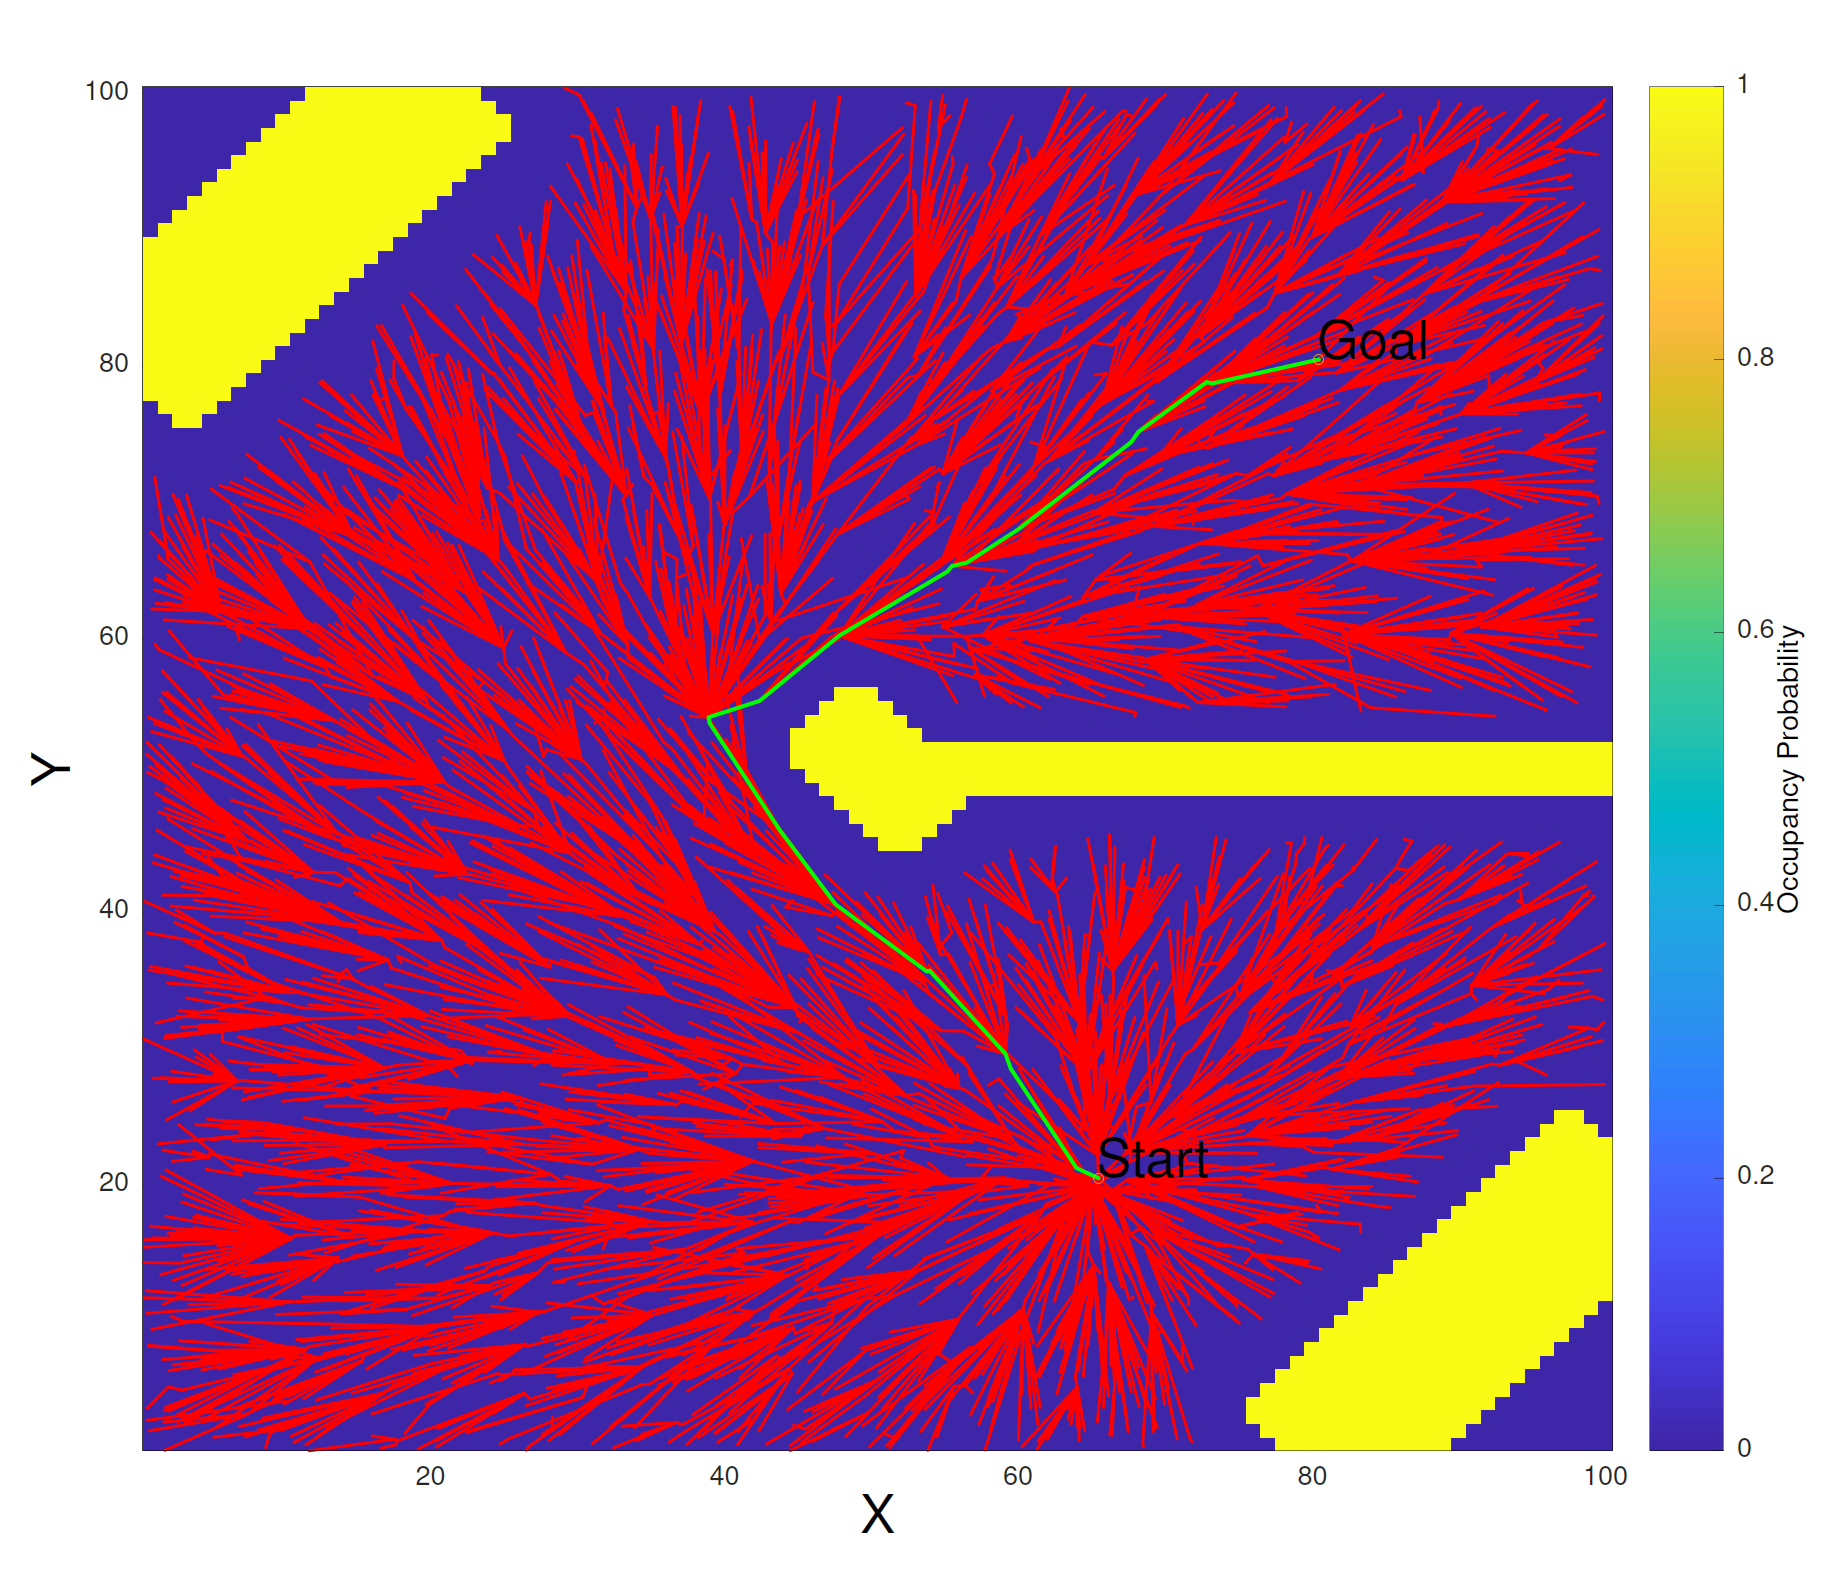
\includegraphics[width=5in]{ExRRTStar.png} % Adjust width as needed
    \caption{3D results using ELQR provided by van den} % Caption for figure
    \label{fig:one} % Label for referencing in text
\end{figure}

\section{Conclusion}




\bibliographystyle{plain}
\bibliography{References}

\end{document}

